\documentclass[12pt,a4paper,russian]{article}

\sloppy

\usepackage[small]{complexity}
\usepackage{csquotes}
\usepackage[russian,english]{babel}
\usepackage{amssymb}
\usepackage{amsmath}
\usepackage{amsthm}
\usepackage{verbatim}
\usepackage{comment}
\usepackage{bookmark}
\usepackage{mathtools}
\usepackage{makecell,xcolor}
\usepackage{tikz}
\usepackage[backend=biber,style=alphabetic]{biblatex}

\usepackage{forloop}

\usepackage[left=2cm,right=2cm,top=2cm,bottom=2cm,bindingoffset=0cm]{geometry}
\usepackage{fancybox,fancyhdr}
\usepackage{lastpage}
\usepackage{titling}

\usepackage{fontspec}

\setmainfont[Ligatures={TeX,Historic}]{CMU Serif}
\setsansfont{CMU Sans Serif}
\setmonofont[Scale=MatchLowercase]{Fira Code}[
	Contextuals=Alternate  % Activate the calt feature
]

\usepackage{minted}

\renewcommand\theFancyVerbLine{\normalsize\arabic{FancyVerbLine}}

\setminted[bash]{breaklines, linenos}
\setminted[text]{breaklines, linenos}
\setminted[cpp]{breaklines, linenos}
\setminted[py3]{breaklines, linenos}

\DeclarePairedDelimiter\set{\lbrace}{\rbrace}
\DeclarePairedDelimiter\abs{\lvert}{\rvert}
\DeclarePairedDelimiter\ceil{\lceil}{\rceil}
\DeclarePairedDelimiter\floor{\lfloor}{\rfloor}

\DeclarePairedDelimiterX{\map}[2]{\lbrace}{\rbrace}{#1 \,\delimsize\vert\,\mathopen{} #2}

\title{Team Reference}
\author{SPb SU ?5 (Belichenko, Gaevoi, Petrov)}

\pagestyle{fancy}
\fancyhead[L]{\theauthor}
\fancyhead[C]{}
\fancyhead[R]{Page {\thepage} of \pageref{LastPage}}
\fancyfoot[L]{}
\fancyfoot[C]{}
\fancyfoot[R]{}

\def\sqgrid{
	\newpage

	\begin{figure} \centering \tikz{
			\foreach \x in {0,...,50} { % вот тут количество строк
				\draw[color=gray,opacity=0.45] (0, 0.5 * \x cm) -- (17, 0.5 * \x cm);
				}
				\foreach \x in {0,...,34} { % вот тут количество столбцов
					\draw[color=gray,opacity=0.45] (0.5 * \x cm, 0) -- (0.5 * \x cm, 25);
					}
	} \end{figure}
}

\def\dotgrid{
	\newpage

	\begin{figure} \centering \tikz{
			\foreach \x in {0,...,50} {
				\foreach \y in {0,...,34} {
					\fill[fill=gray,opacity=0.45] (0.5 * \y cm, 0.5 * \x cm)
					node{\textcolor{gray}{.}};
					};
					}
	} \end{figure}
}

\begin{document}

\selectlanguage{russian}

\tableofcontents

\section{Setup \& Scripts}

\subsection{CMake}

\inputminted{text}{code/CMakeLists.txt}

\subsection{wipe.sh}

\inputminted{bash}{code/wipe.sh}

\subsection{Stack size \& Profiling}

\inputminted{bash}{code/stack.sh}

\section{Language specific}

\subsection{C++}

\subsubsection{G++ builtins}

\begin{itemize}
	\item \mintinline{C++}{__builtin_popcount(x)}~--- количество единичных бит в двоичном представлении 32-битного (знакового или беззнакового) целого числа.
	\item \mintinline{C++}{__builtin_popcountll(x)}~--- то же самое для 64-битных типов.
	\item \mintinline{C++}{__builtin_ctz(x)}~--- количество нулей на конце двоичного представления 32-битного целого числа. Например, для $5$ вернётся $0$, для $272 = 256 + 16$ --- $4$ и т. д. Может не работать для нуля (вообще не стоит вызывать для $x = 0$, по-моему это и упасть может).
	\item \mintinline{C++}{__builtin_ctzll(x)}~--- то же самое для 64-битных типов.
	\item \mintinline{C++}{__builtin_clz(x)}~--- количество нулей в начале двоичного представления 32-битного целого числа. Например, для $2^{31}$ или $-2^{31}$ вернётся
		$0$, для $1$ --- $31$ и т. д. Тоже не надо вызвывать с $x = 0$.
	\item \mintinline{C++}{__builtin_clzll(x)}~--- то же самое для 64-битных типов.

	\item \mintinline{C++}{bitset<N>._Find_first()}~--- номер первой позиции с единицей в битсете или его размер
		(то есть $N$), если на всех позициях нули.
	\item \mintinline{C++}{bitset<N>._Find_next(x)}~--- номер первой позиции с единицей среди позиций с номерами строго больше $x$; если такой нет, то $N$.
\end{itemize}

\subsubsection{hash}

\inputminted{C++}{code/hacks.cpp}

\subsection{Python}

\inputminted{Python}{code/python.py}

% \section{Bugs}

\begin{itemize}
	\item \texttt{powmod} :)

	\item Всегда чекать Куна дважды, особенно на количество итераций

	\item \texttt{uniform\_int\_distribution} от одного параметра

	\item \texttt{for (char c : "NEWS")}

	\item Порядок верхних и нижних границ в случае, когда задача двумерна
		$t - b \neq b - t$

	\item static с мультитестами

	\item set со своим компаратором склеивает элементы

	\item Два вектора с соответствующими элементами, сортим один, а элементы
		второго ссылаются на чушь. Предлагается лечить заведением структуры с
		компаратором на каждый чих. В целом, для этого можно написать навороченную
		хрень на шаблонах.

	\item В графе с вершинами степени не больше одного надо писать выделение
		цикла полностью, срезать угол на какой-нибудь тупой меморизации, потому
		что кажется, что он может выглядеть только одним или несколькими
		какими-нибудь специальными способами, не получится, а дебажить сложно.

	\item Структуры, основанные на указателях, не стоит хранить в векторах.

	\item В Карасе для того, чтобы перейти в подстроку, надо сначала идти в
		родителя, а только потом по суфф. ссылкам, эти вещи не коммутируют.

	\item Когда ходим большим количеством указателей по циклу, на единицу
		сдвигается только первый указатель, а остальные могут сдвинуться на много.

	\item \texttt{string str(str2, 'x'); str = 'a';}
\end{itemize}

\section{Geometry}

\subsection{Пересечение прямых}

\begin{equation*}
    AB = A - B; CD = C - D
\end{equation*}
\begin{equation*}
    (A \times B \cdot CD.x - C \times D \cdot AB.x : A \times B \cdot CD.y - C \times D \cdot AB.y : AB \times CD)
\end{equation*}

\subsection{Касательные}

Точки пересечения общих касательных окружностей с центрами в $(0, 0)$ и $(x, 0)$ равны $\frac{x r_1}{r1 \pm r2}$.
$x$ координата точек касания из $(x, 0)$ равна $\frac{r^2}{x}$.

\subsection{Пересечение полуплоскостей}

Точно так же, как в выпуклой оболочке, но надо добавить bounding box (квадратичного размера относительно координат на входе) и завернуть два раза.
Ответ можно найти как подотрезок от первой полуплоскости типа true до нее же самой на втором круге.
Проверку на вырожденность лучше делать простой проверкой пары-тройки точек из предполагаемого ответа. Стоит быть аккуратнее с точностью.

\section{Template dsu}

\inputminted{cpp}{code/dsu.cpp}

\section{Numbers}

\begin{itemize}
	\item A lot of divisors
		\begin{itemize}
			\item $\leq 20: d(12)=6$
			\item $\leq 50: d(48)=10$
			\item $\leq 100: d(60)=12$
			\item $\leq 10^3: d(840)=32$
			\item $\leq 10^4: d(9240)=64$
			\item $\leq 10^5: d(83160)=128$
			\item $\leq 10^6: d(720720)=240$
			\item $\leq 10^7: d(8648640)=448$
			\item $\leq 10^8: d(91891800)=768$
			\item $\leq 10^9: d(931170240)=1344$
			\item $\leq 10^{11}: d(97772875200)=4032$
			\item $\leq 10^{12}: d(963761198400)=6720$
			\item $\leq 10^{15}: d(866421317361600)=26880$
			\item $\leq 10^{18}: d(897612484786617600)=103680$
		\end{itemize}

	\item Numeric integration
		\begin{itemize}
			\item simple: $F(0)$
			\item simpson: $\frac{F(-1) + 4 \cdot F(0) + F(1)}{6}$
			\item runge2: $\frac{ F(-\sqrt{\frac{1}{3}}) + F(\sqrt{\frac{1}{3}}) }{2}$
			\item runge3: $\frac{ F(-\sqrt{\frac{3}{5}}) \cdot 5 + F(0) \cdot 8 +  F(\sqrt{\frac{3}{5}}) \cdot 5}{18}$
		\end{itemize}
\end{itemize}	

% \section{Graphs}

\subsection{Weighted matroid intersection}
\lstinputlisting[language=C++]{code/weighted_matroid_intersection.cpp}


\section{Push-free segment tree}

\lstinputlisting[language=C++]{code/pushfreesegtree.cpp}

\section{Number theory}

\subsection{Chinese remainder theorem without overflows}

\inputminted{cpp}{code/crt.cpp}

\subsection{Integer points under a rational line}

\inputminted[mathescape]{cpp}{code/under_line.cpp}

\section{Suffix Automaton}

\lstinputlisting[language=C++]{code/maximalist_tomato.cpp}

\section{Palindromic Tree}

\lstinputlisting[language=C++]{code/palindromic_tree.cpp}


\section{Smth added at last moment}

\subsection{Dominator Tree}

\inputminted{cpp}{code/dominator_tree.cpp}

\subsection{Suffix Array}

\inputminted{cpp}{code/suffix_array.cpp}

\subsection{Fast LCS}

\inputminted{cpp}{code/fast_lcs.cpp}

\subsection{Fast Subset Convolution}

\inputminted{cpp}{code/fast_subset_convolution.cpp}

\section{Karatsuba}

\inputminted{C++}{code/Karatsuba.cpp}

\section{Two Strong Chinese}

\inputminted[firstline=228, lastline=369]{cpp}{code/2StrongChinese.cpp}

\section{OEIS}

\subsection{Числа Белла}

1, 1, 2, 5, 15, 52, 203, 877, 4140, 21147, 115975, 678570, 4213597, 27644437, 190899322, 1382958545, 10480142147, 82864869804, 682076806159, 5832742205057, 51724158235372, 474869816156751, 4506715738447323, 44152005855084346, 445958869294805289, 4638590332229999353, 49631246523618756274

\subsection{Числа Каталана}

1, 1, 2, 5, 14, 42, 132, 429, 1430, 4862, 16796, 58786, 208012, 742900, 2674440, 9694845, 35357670, 129644790, 477638700, 1767263190, 6564120420, 24466267020, 91482563640, 343059613650, 1289904147324, 4861946401452, 18367353072152, 69533550916004, 263747951750360, 1002242216651368, 3814986502092304


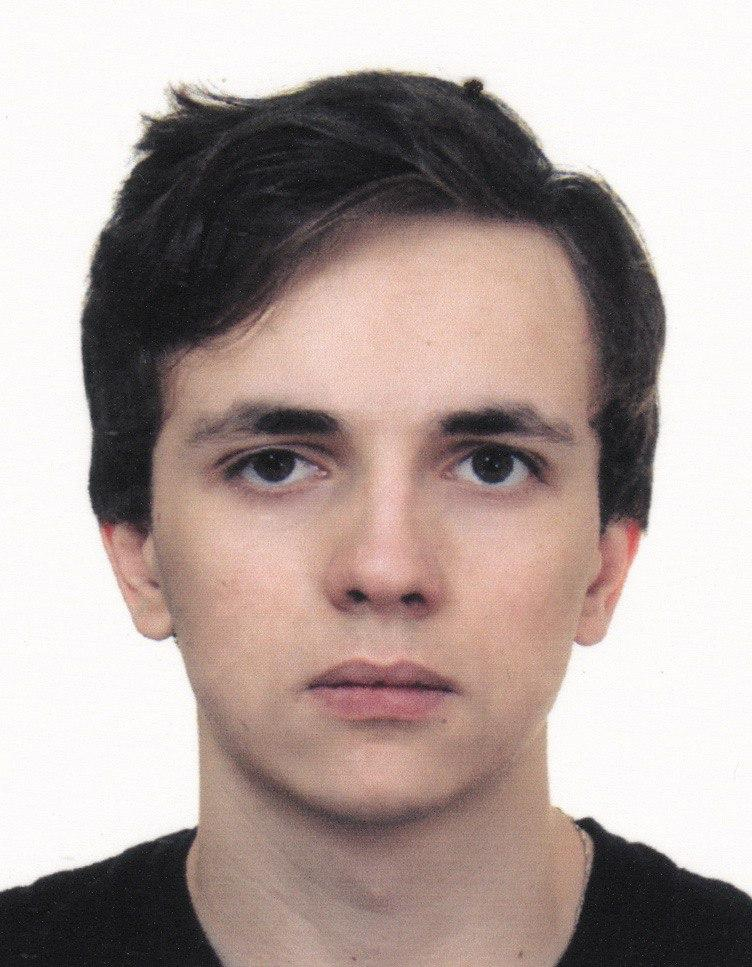
\includegraphics[width=\linewidth]{Belik}

\newpage

\newcounter{ct}

\forloop[2]{ct}{\thepage}{\value{ct} < 24}{%
	\sqgrid%
	\dotgrid%
	}

\end{document}
